\documentclass[a4paper]{article}

%====================== PACKAGES ======================

\usepackage[french]{babel}
\usepackage[utf8x]{inputenc}
%pour gérer les positionnement d'images
\usepackage{float}
\usepackage{amsmath}
\usepackage{amssymb}
\usepackage{mathtools}
\usepackage{graphicx}
\usepackage[colorinlistoftodos]{todonotes}
\usepackage{url}
%pour les informations sur un document compilé en PDF et les liens externes / internes
\usepackage{hyperref}
%pour la mise en page des tableaux
\usepackage{array}
\usepackage{tabularx}
%pour utiliser \floatbarrier
%\usepackage{placeins}
%\usepackage{floatrow}
%espacement entre les lignes
\usepackage{setspace}
%modifier la mise en page de l'abstract
\usepackage{abstract}
%police et mise en page (marges) du document
\usepackage[T1]{fontenc}
\usepackage[top=2cm, bottom=2cm, left=2cm, right=2cm]{geometry}
%Pour les galerie d'images
\usepackage{subfig}
%landscape
\usepackage{pdflscape}

%====================== INFORMATION ET REGLES ======================

%rajouter les numérotation pour les \paragraphe et \subparagraphe
% \setcounter{secnumdepth}{4}
% \setcounter{tocdepth}{4}

\hypersetup{							% Information sur le document
pdfauthor = {Guillaume Clochard
			Thomas Coquereau},			% Auteurs
pdftitle = {Mini-Projet d'Intelligence Artificiel
			Emploi du temps à Polytech Nantes},			% Titre du document
pdfsubject = {Compte Rendu Mini-Projet},		% Sujet
pdfkeywords = {},	% Mots-clefs
pdfstartview={FitH}}					% ajuste la page à la largueur de l'écran
%pdfcreator = {MikTeX},% Logiciel qui a crée le document
%pdfproducer = {}} % Société avec produit le logiciel

%======================== DEBUT DU DOCUMENT ========================

\begin{document}

% %régler l'espacement entre les lignes
% \newcommand{\HRule}{\rule{\linewidth}{0.5mm}}
% %espacement entre les lignes d'un tableau
% \renewcommand{\arraystretch}{1.5}

\title{Mini-Projet d'Intelligence Artificiel \\
    Emploi du temps à Polytech Nantes}
\author{Guillaume Clochard, Thomas Coquereau}
\maketitle

% \tableofcontents

% \thispagestyle{empty}
% \setcounter{page}{0}
%ne pas numéroter le sommaire

%====================== INCLUSION DES PARTIES ======================

\section{Introduction}

Ce rapport présente un premier travail effectué dans le cadre du Mini-Projet
d'Intelligence Artificielle.
Il consiste en la planification de l'emploi du temps à Polytech Nantes.
Ce premier rendu s'attarde sur la modélisation générale du problème ainsi qu'une
première proposition de solution.


\newpage

\section{UML}
\begin{center}
	\begin{figure}[t]
	   \caption{\label{1} Diagramme de classe}
	   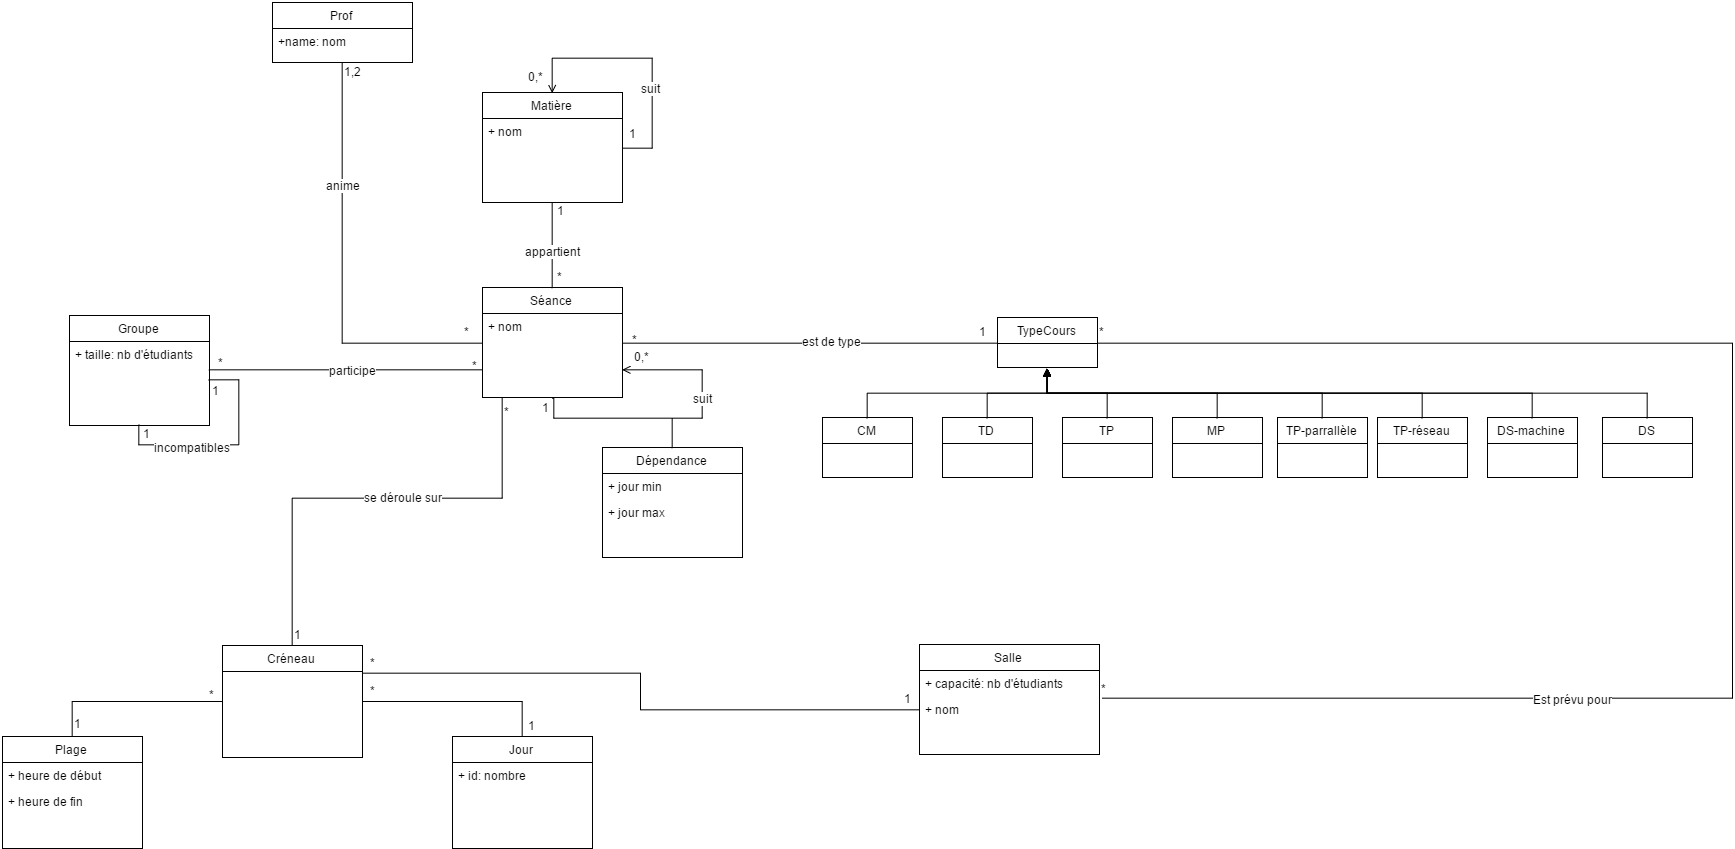
\includegraphics[keepaspectratio=true,width=17cm]{diagrammeClasse.png}
	\end{figure}
\end{center}
Voici le diagramme de classe décrivant les données nécessaires à la gestion de l'emploi du temps.
Comme on peut le constater, on regroupe l'ensemble des données nécessaires et déterminées à l'avance dans des Séances. A savoir : le(s) groupe(s) d'étudiants concerné(s), le professeur, la matière, ainsi que le type de cours. Ensuite ces séances vont être associées à des créneaux par notre solution. Les créneaux étant le regroupement d'un jour, une plage horaire et une salle.
Un peu noter des détails intéressants, sur Groupe, il y a la notion d'incompatibilité qui permet de définir lorsqu'il est possible pour deux groupes d'avoir cours sur une même plage horaire. Sur matière on à la notion de suite, lorsqu'une matière débute après la fin d'une autre (cf Mini-Projet d'IA qui suit le cours d'IA). Et enfin sur séance, on a la notion de suite aussi qui décrit une nombre de jours minimum et maximum avant le prochain cours de la même matière.
\newpage

\section{Instance}

Le problème modélisé, il convient maintenant de construire un jeu de données qui
servira à la construction de l'emploi du temps.

La Figure \ref{fig:objet} représente sous forme de diagramme objet l'instance
sur laquelle nous allons travailler. Pour des soucis de lisibilité, le diagramme
est incomplet. Il a été choisi de ne représenter que quelques séances et de ne
pas représenter les dépendances entre elles.

L'instance complète est disponible sous format Prolog dans le fichier
\texttt{instance.pl}.

\begin{landscape}

    \begin{figure}[t]
        \includegraphics[keepaspectratio=true,width=26cm]{diagrammeObjet.png}
            \caption{\label{fig:objet} Diagramme objet tronqué}
    \end{figure}

\end{landscape}


\newpage


\section{Solution}

Il convient à présent de définir une première proposition de solution.

Imaginons qu’on dispose d’une fonction $\textsc{Planifier}$ en charge de créer
l’emploi du temps.

Sa signature serait grossièrement :

\begin{description}

\item[Entrées] les séances $S$, les plages horaires $H$, les jours de
travail $J$ et les salles $L$
\item[Sortie] un sous-ensemble de tous les créneaux $C$

\end{description}

\begin{center}

$ \begin{array}{ll}
\textsc{Planifier} : S \times H \times J \times L \quad \not\to \quad C
\end{array}$

\end{center}

On retrouve donc les objets modélisés à la Figure \ref{fig:uml}.

\subsection{Pré-conditions}

Les pré-conditions de la fonction $\textsc{Planifier}$ sont formées par le respect
de la modélisations UML et de l'ajout de détails comme :

\begin{itemize}

    \item les jours sont des nombres entiers appartenant à $\mathbb{N}_{+}$
    \item les plages horaires ne débordent pas des 24h et ne se recouvrent pas

        \[
            \forall(h_0, h_1) \in H, h_0 \leq 0h00, h_1 \leq 23h59
        \]

        \[
            \forall(h_0, h_1),(h_2, h_3) \in H, \;
            h_0 < h_1 \leq h_2 < h_3 \;
            \text{ou} \; h_2 < h_3 \leq h_0 < h_1
        \]

    \item tous les types de cours des séances voient une salle compatible

        \[
            \forall s \in S, \exists l \in L, \text{typeCours}(s) =
            \text{typeCours}(l)
        \]

\end{itemize}

\subsection{Post-conditions}

\begin{itemize}

    \item les créneaux ne débordent pas sur des horaires, des jours ou des
        salles différents des entrés

        \begin{equation}\label{eqn:p1}
            \forall(s, h, j, l) \in \textsc{Planifier}(S, H, L, L),
            s \in S, h \in H, j \in J, l \in L
            \tag{P1}
        \end{equation}

    \item toutes les séances sont affectées à un créneau

        \begin{equation}\label{eqn:p2}
            \forall s \in S,
            \exists(s, h, j, l) \in \textsc{Planifier}(S, H, L, L)
            \tag{P2}
        \end{equation}

    \item toute séance est affectée à une salle qui respecte son type de cours
        et son effectif

        \begin{equation}\label{eqn:p3}
            \forall(s, h, j, l) \in \textsc{Planifier}(S, H, L, L),\;
            \text{typeCours}(s) = \text{typeCours}(l)
            \  \text{et} \  \text{effectif}(s) \leq \text{taille}(l)
            \tag{P3}
        \end{equation}

    \item un enseignant n'a pas deux séances en même temps

        \begin{equation}\label{eqn:p4}
            \forall(s_1, h, j, l_1), (s_2, h, j, l_2)
            \in \textsc{Planifier}(S, H, L, L),\;
            \text{prof}(s_1) \not= \text{prof}(s_2)
            \tag{P4}
        \end{equation}

    \item des groupes incompatibles n'ont pas cours en même temps

        \begin{equation}\label{eqn:p5}
            \begin{split}
                & \forall(s_1, h, j, l_1), (s_2, h, j, l_2)
                \in \textsc{Planifier}(S, H, L, L),\;\\
                & \lnot\text{incompatibles}(g_1, g_2)
                \quad \forall g_1 \in groupes(s_1), \forall g_2 \in groupes(s_2)
            \end{split}
            \tag{P5}
        \end{equation}

    \item les créneaux respectent le séquencement des séances et des matières

        \begin{equation}\label{eqn:p6}
            \begin{split}
                & \forall(s_1, h_1, j_1, l_1), (s_2, h_2, j_2, l_2)
                \in \textsc{Planifier}(S, H, L, L),
                \text{tel que} \  \text{suit}(s_2, s_1)\\
                & \text{alors} \  j_2 \in O
                \  \text{où} \  O = intervalleJours(s_1, s_2)\\
                & \text{et si} \  j_2 = j_1 \  \text{alors} \  h_2 > h_1
            \end{split}
            \tag{P6}
        \end{equation}

\end{itemize}

\subsection{Algorithme non déterministe}

Nous avons choisit de formuler notre solution sous forme d'un algorithme non déterministe.

\begin{algorithm}                    
\caption{basique}      
\label{alg1}                           
\begin{algorithmic}                    % enter the algorithmic environment
    \REQUIRE $C = \emptyset$
    \WHILE{$|S| > 0$}
        \STATE $s \Leftarrow choix_nd(S)$
        \STATE $h \Leftarrow choix_nd(H)$
        \STATE $j \Leftarrow choix_nd(J)$
        \STATE $l \Leftarrow choix_nd(L)$
        \STATE $C \Leftarrow (s, h, j, l)$
        \IF{les conditions sont respectées avec $c$}
            \STATE $C \Leftarrow c \cup C$
            \STATE $S \Leftarrow S / s$
        \ELSE
            \STATE $retourner \perp$
        \ENDIF
    \ENDWHILE
\end{algorithmic}
\end{algorithm}

\newpage

\end{document}
